%---------------------------------------------------------------------
%
%                          Cap�tulo 4
%
%---------------------------------------------------------------------
%
% 04Imagenes.tex
% Copyright 2009 Marco Antonio Gomez-Martin, Pedro Pablo Gomez-Martin
%
% This file belongs to the TeXiS manual, a LaTeX template for writting
% Thesis and other documents. The complete last TeXiS package can
% be obtained from http://gaia.fdi.ucm.es/projects/texis/
%
% Although the TeXiS template itself is distributed under the 
% conditions of the LaTeX Project Public License
% (http://www.latex-project.org/lppl.txt), the manual content
% uses the CC-BY-SA license that stays that you are free:
%
%    - to share & to copy, distribute and transmit the work
%    - to remix and to adapt the work
%
% under the following conditions:
%
%    - Attribution: you must attribute the work in the manner
%      specified by the author or licensor (but not in any way that
%      suggests that they endorse you or your use of the work).
%    - Share Alike: if you alter, transform, or build upon this
%      work, you may distribute the resulting work only under the
%      same, similar or a compatible license.
%
% The complete license is available in
% http://creativecommons.org/licenses/by-sa/3.0/legalcode
%
%---------------------------------------------------------------------

\chapter{Implementaci\'on y Especificaci\'on}
\label{cap4}
\label{cap:implentacion-especificacion}


\begin{FraseCelebre}
\begin{Frase}
%El alma nunca piensa sin una imagen mental.
\end{Frase}
\begin{Fuente}
%Arist�teles
\end{Fuente}
\end{FraseCelebre}

%-------------------------------------------------------------------
\section{Introducci\'on}
%-------------------------------------------------------------------
\label{cap4:sec:intro}

Una vez decididas las herramientas que se iban a usar y con gran parte de la informaci\'on recogida, lleg\'o el momento de realizar un an\'alisis del funcionamiento de Android y dise\~nar un protocolo de red que ayudase a conectar la aplicaci\'on de Android con el juego de Unity. En este cap\'itulo se explicar\'an todas las decisiones que se tomaron a la hora de implementar ambas aplicaciones y se ampliar\'a la informaci\'on sobre como interactuan ambos sistemas.

%-------------------------------------------------------------------
\section{Aplicaci\'on Android}
%-------------------------------------------------------------------
\label{cap4:sec:Android}


Como se ha comentado en cap\'iyulos anteriores, se ha usado Android Studio como entorno de desarrollo de la aplicaci\'on m\'ovil. Para poder comenzar este desarrollo primero se ha tenido que comprender el funcionamiento de un dispositivo Android y para eso primero se debe conocer el ciclo de vida de una aplicaci\'on cuando es ejecutada en un dispositivo Android:

\begin{figure}[h]

\centering {
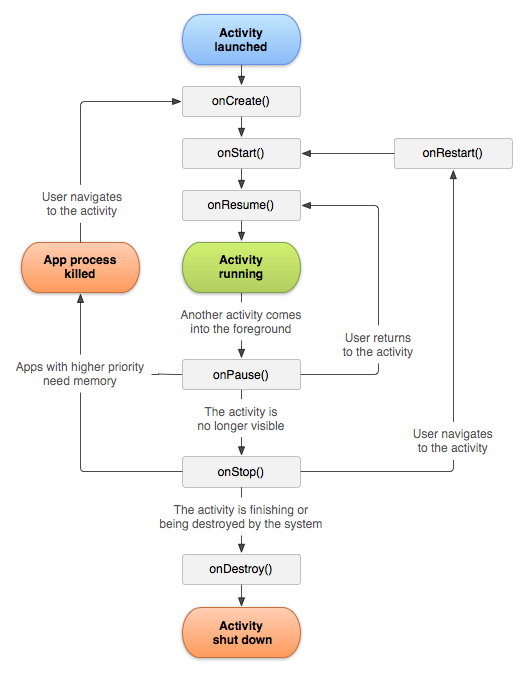
\includegraphics[width=0.6\textwidth]{Imagenes/Bitmap/Ciclo_de_vida_Android.png}
}
\end{figure}

Con este ciclo de vida en mente, hay que tener en cuenta que una vez la aplicaci\'on quedase en pausa porque entrase una llamada o simplemente el usuario dejase la aplicaci\'on en segundo plano, Android podr\'ia matar el proceso de nuestra aplicaci\'on y tener que volver a crearla si el usuario vuelve a poner en la vista principal la aplicaci\'on.
\\
En Android es necesario definir las acciones que el sistema va a ejecutar cuando estos estados del ciclo de vida se inicien. Para el caso espec\'ifico de este proyecto se vi\'o que al querer usar la c\'amara nada m\'as iniciar la aplicaci\'on, era necesario utilizar 2 actividades diferentes. La primera de estas actividades se ejecuta siempre que la aplicaci\'on se inicia ya que su funci\'on es la de utilizar la c\'amara para poder leer un c\'odigo QR. Este c\'odigo QR contiene 2 datos:

\begin{enumerate}

\item IP del ordenador al que debe conectarse.
\item Puerto al que deben enviarse los paquetes.

\end{enumerate}

La creaci\'on del QR y la utilizaci\'on de la libreria ZXing\footnote{https://archive.codeplex.com/?p=zxingnet} se explican en este mismo cap\'itulo pero en el apartado de  IMPLEMENTACION DE LA APLICAICON DE ESCRITORIO.
\\
Gracias a la API de Android, se ha podido acceder al manejo completo de la c\'amara. Esta implementaci\'on se encuentra en el paquete:\\ \textbf{com.google.android.gms.vision.CameraSource.}\footnote{https://developers.google.com/android/reference/com/google/android/gms/vision/CameraSource?hl=es}
\\
Adem\'as de la importaci\'on de paquetes, Android tiene un sistema de gesti\'on de permisos. Para poder usar la c\'amara es necesario a\~nadirlos expl\'icitamente en el archivo \textbf{AndroidManifest.xml:}\footnote{https://developer.android.com/guide/topics/manifest/manifest-intro?hl=es-419}
\\    <uses-permission android:name="android.permission.CAMERA" />\\


Desde el punto del desarrolador, para poder utilizar esta herramienta va a ser necesario tener la versi\'on XX.XX de Unity3D y Android Studio en su versi\'on XX.XX y un tel\'efono m\'ovil que podamos utilizar como emulador.
\\
Esta herramienta tiene 2 partes que est\'an diferenciadas por la plataforma para las que van destinadas. En el lado de PC, se ha implementado una serie de clases que son independientes al juego. 
Estas clases est\'an escritas en C\# y utilizan las librer\'ias  nativas de red de este lenguaje para comunicaci\'on. Por encima de estas clases se encuentra la parte espec\'ifica de Unity3D que facilita su uso. 
\\
Como parte extra a la herramienta, se ha propuesto un inicio de conexi\'on a trav\'es de la lectura de un QR. Con esto lo que se pretende es enlazar el dispositivo Android con el juego que se est\'a ejecutando en Unity. 
La lectura de este QR se hace directamente desde la aplicaci\'on creada para este proyecto. Al leer el QR y emparejarse ambos dispositivos, la aplicaci\'on Android cambia de c\'amara a mando.
\\

[INSERTE IMAGEN DE ARQUITECTURA Y DIAGRAMA DE CLASES Y COMPONENTES  + EXPLICACION]


%-------------------------------------------------------------------
\section{Protocolo de conexi\'on}
%-------------------------------------------------------------------
\label{cap4:sec:protocolo}

La conexi\'on se incia con la lectura de un QR que se mostrar\'a en el juego ejecutado en Unity. Una vez el dispositivo Android haya leido ese QR, Android manda la resoluci\'on del dispositivo con 2 bytes. 
El servidor que se est\'a ejecutando en Unity, guarda esa informaci\'on y escala el mando que se haya seleccionado a la resoluci\'on que tiene el dispositivo Android. Una vez hecho esto, se calculan las coordenadas de los botones del mando y se pasan a un XML.
\\
Este XML junto a la imagen es enviado al dispositivo Android. El tel\'efono guarda esta informaci\'on y deja de mostrar la c\'amara para mostrar la imagen del mando que se le ha enviado. En la aplicaci\'on Android han quedado guardadas las coordenadas de los botones, por lo que ya podr\'ia empezar la sesi\'on de juego.
\\
Durante una sesi\'on de juego estandar, el dispositivo Android recibir\'a pulsaciones del jugador en la pantalla, calcular\'a el bot\'on al que corresponde y enviar\'a al ordenador un array de 10 bytes en los que ir\'a la informaci\'on necesaria para saber la acci\'on que ha hecho el jugador y reaccionar consecuentemente.
\\

[ADJUNTAR IMAGEN DESCRIPTIVA DEL CONTENIDO DEL ARRAY + POSTERIOR EXPLICACION DEL SIGNIFICADO DE CADA COSA Y LOS VALORES QUE PUEDE TOMAR]

%-------------------------------------------------------------------
\section{El uso de los QR para inicio de conexi\'on}
%-------------------------------------------------------------------
\label{cap4:QR}

Los QR's son los c\'odigos de barras 2D, la raz\'on por la que se ha elegido esta tecnolog\'ia para sincronizar el dispositivo Android con el juego en ejecuci\'on en Unity es debido a que es una tecnolog\'ia que ambos sistemas saben interpretar y porque actualmente es un est\'andar, a parte nuestro usuarios ya tienen el propio dispositivo m\'ovil en sus manos listo para sincronizar y pasar a ser su mando. En la mayor parte de ocasiones, este contenido es una URL espec\'ifica, en el caso de este proyecto, lo que contiene el QR es la direcci\'ion IP del equipo que est\'a ejecutando el juego de Unity. A su vez contiene el puerto donde el dispositivo Android debe conectarse y mandar sus mensajes. Una vez leido el QR, la aplicaci\'on Android guarda estos datos para que el juego pueda comenzar y el QR pueda desaparecer. 
\\

%-------------------------------------------------------------------
\section{Pantalla secundaria y controlador}
%-------------------------------------------------------------------
\label{cap4:pantallasecundaria}

Como se dijo en el cap\'itulo 2, para este proyecto se ha usado de referencia las consolas Wii U de Nintendo y PlayLink de Sony. Se quiere que los desarrolladores de los juegos hecho en Unity pudiesen mostrar elementos del juego como un mapa, un inventario o unas notas que seguir fuera del HUD de juego para que este no se viese saturado.
\\
Es por esta idea, por lo que a la aplicaci\'on de Android se le ha dado la capacidad de recibir im\'agenes y mostrarlas por la pantalla del Android. Con esto se da la posibilidad de enviar una im\'agen que ya haya sido creada con anterioridad o incluso se abre la posibilidad de enviar lo que est\'a renderizando una c\'amara dentro del juego en tiempo real y hacer que nuestro dispositivo Android lo muestre. 
\\
Esto lo que implica es que la comuncicaci\'on entre la aplicaci\'on Android y el juego de Unity va a ser constante y se corre el riesgo de saturar la red. Para solventar este posible fallo, se decidi\'o comprimir la imagen que se enviaba a formato PNG. Este formato fue el elegido porque tanto Unity como Android dan soporte de compresi\'on y descompresi\'on de manera eficaz. 



% Variable local para emacs, para  que encuentre el fichero maestro de
% compilaci�n y funcionen mejor algunas teclas r�pidas de AucTeX
%%%
%%% Local Variables:
%%% mode: latex
%%% TeX-master: "../ManualTeXiS.tex"
%%% End:
